\section{Ensemble Methods}

\smallskip \hrule height 2pt \smallskip

Vocab
\begin{itemize}
	\item \textbf{decision tree stump}: 
	\item \textbf{decision stub}:  (used in lecture 10 pg 14: boosting)  ?? horizontal or vertical line only?  
	\item \textbf{axis aligned classifier}
\end{itemize}

Instead of learning a single classifier, learn many weak classifiers that are good at different parts of the data. 
The output class is a weighted vote of each classifier. 
\begin{itemize}
	\item classifiers that are most "sure" will vote with more conviction
	\item classifiers will be most "sure" about a particular part of the space. 
	\item on average, these will do better than a single classifier. 
\end{itemize}

% transcribed understanding of audio from week 8
This is better than breaking up the space into a bunch of sub-spaces and making single classifiers for each.  
If you had single classifiers for sub-spaces, you would be losing information about the surroundings.
It is better to have all classifiers cover the whole space, but let them vote. 

\subsection{Bagging vs Boosting}
\textbf{Bagging:} % http://stats.stackexchange.com/questions/18891/bagging-boosting-and-stacking-in-machine-learning
\begin{itemize}
	\item parallel ensemble: each model is built independently
	\item aim to decrease variance, not bias
	\item suitable for high variance low bias models (complex models)
	\item \textbf{samples are drawn with replacement}
	\item each model in the ensemble vote with equal weight % https://en.wikipedia.org/wiki/Ensemble_learning
	\item an example of a tree based method is random forest, which develop fully grown trees (note that RF modifies the grown procedure to reduce the correlation between trees)
\end{itemize}

\textbf{Boosting:}  % http://stats.stackexchange.com/questions/18891/bagging-boosting-and-stacking-in-machine-learning
\begin{itemize}
	%\item sequential ensemble: try to add new models that do well where previous models lack
	\item \textbf{incrementally building an ensemble by training each new model instance to emphasize the training instances that previous models mis-classified.} 
	\item aim to decrease bias, not variance
	\item suitable for low variance high bias models
	\item an example of a tree based method is gradient boosting
	\item In some cases, boosting has been shown to yield better accuracy than bagging, but it also tends to be more likely to over-fit the training data. % https://en.wikipedia.org/wiki/Ensemble_learning
	\item AdaBoost is the most common
\end{itemize}


\subsection{Bagging}
\textbf{"Bagging" = \underline{B}ootstrap \underline{AGG}regation.}
For $i = 1, 2, \dots, K$:   (?? translate to english ??) 
\begin{itemize}
	\item $T_i \leftarrow$ randomly select $M$ training instances with replacement.
	\item $h_i \leftarrow$ learn($T_i$)
\end{itemize}
Then combine the $h_i$ together with uniform voting ($w_i = 1/K$ for all $i$).

\subsubsection{Example: CART decision boundary}
CART is a decision tree learning algorithm. \hfill \\

100 bagged trees:  shades of blue/red indicate the strength of votes for particular classifications. \hfill \\
Picked random subsets of the data, and built classifiers.  These classifiers are weighted!! \hfill \\  % week 8 audio
?? (not the strength of different classifiers.)   \hfill \\ 
?? Is white an overall uncertain vote ??   \hfill \\ 
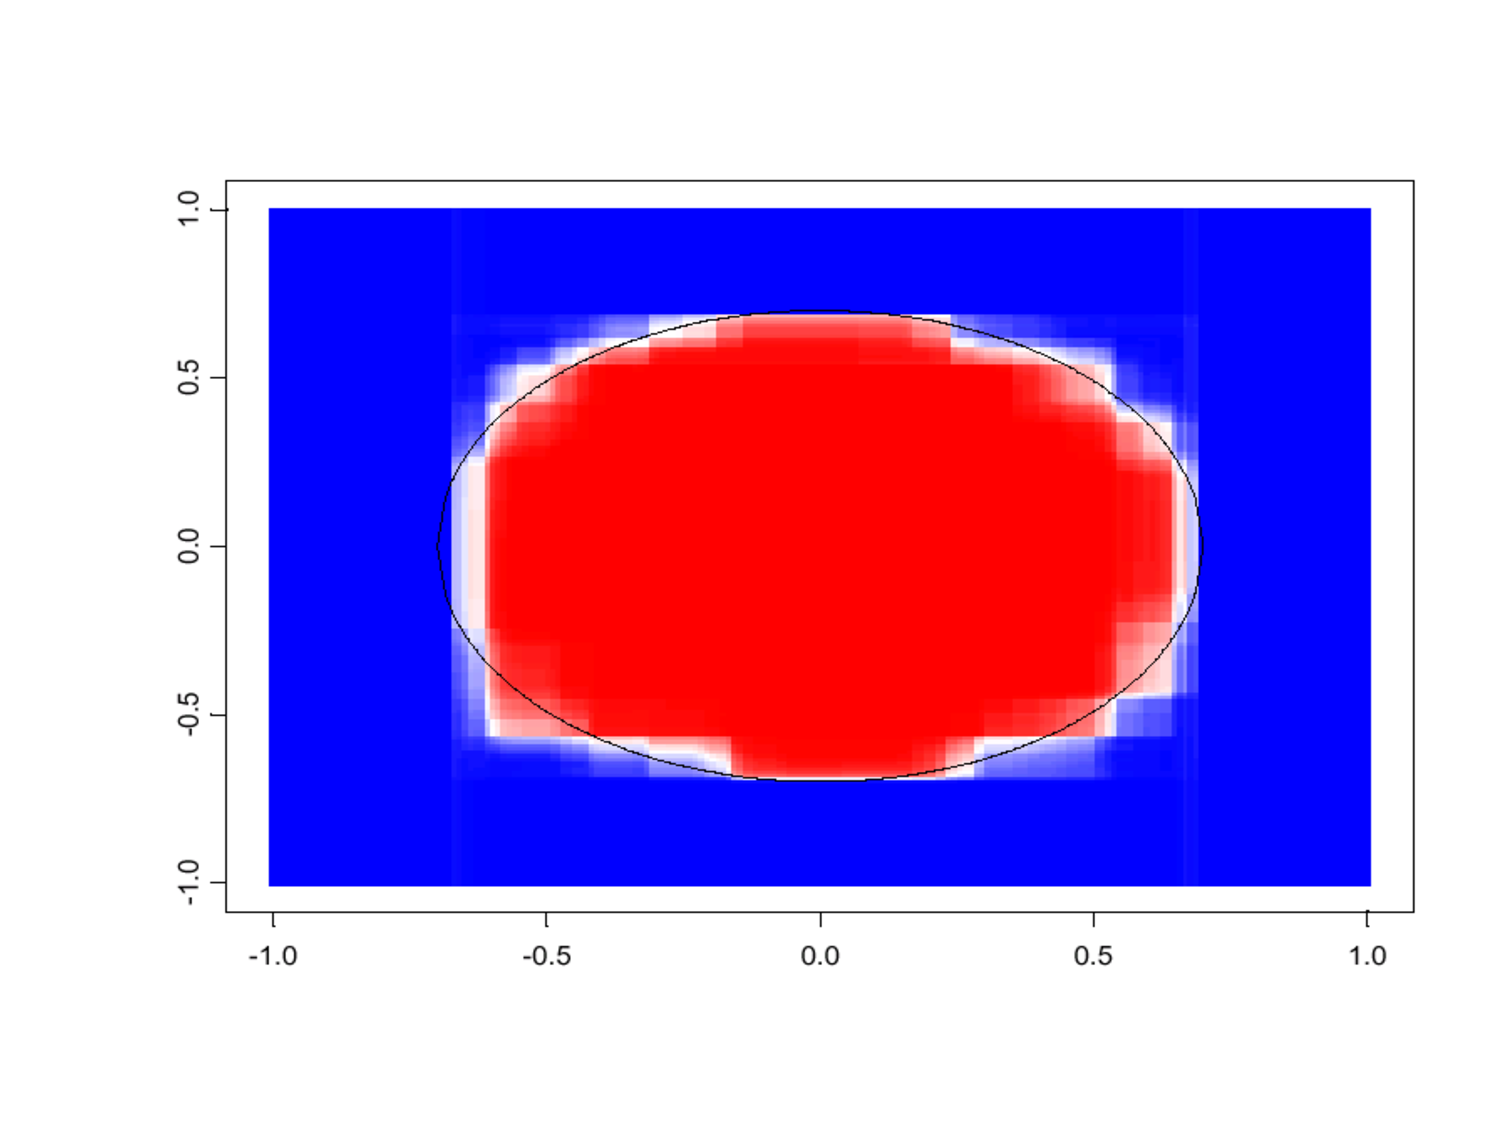
\includegraphics[width=2in]{figures/100_bagged_trees.pdf} \hfill \\
Approximating the circle with a set of lines.  Piecewise linear functions. \hfill \\ % wk 8 audio
The more trees you have, the smoother the boundary will be. 

\subsubsection{Fighting the bias-variance tradeoff}
Simple (a.k.a. weak) learners are good. \hfill \\ 
Examples of weak learners we can use: \hfill \\ 
Naive Bayes, logistic regression, perceptron, decision stumps, shallow decision trees, etc. \hfill \\ 
These learners have low variance; they don't usually overfit. 

But simple (a.k.a. weak) learners are also bad: \hfill \\ 
They have high bias (high error), so you can't solve hard learning problems. \hfill \\ 

The solution: Boosting. 

\subsection{Boosting}

\begin{itemize}
	\item Combine	weak	classifiers	to get very strong classifier.  
		The weak classifiers only have to be slightly better than random on the training data. 
		You end up with a very strong classifier.  You can get zero training error. 
	\item AdaBoost is the most common algorithm
	\item Similar to logistic regression:
		\begin{itemize}
			\item both linear models.  Boosting "learns" features.  
			\item similar loss functions
			\item single optimization (Logistic Regression) versus incrementally improving classification (Boosting) 
		\end{itemize}
	\item  boosting with a weak classifier is better than using a fancy classifier. 
		A boosted version will always do better than the vanilla one. 
	\ 
\end{itemize}


An approach to calculate the output using several different models and then average the result using a weighted average approach. 
By combining the advantages and pitfalls of these approaches by varying your weighting formula you can come up with a good predictive force for a wider range of input data, using different narrowly tuned models.  % http://stats.stackexchange.com/questions/18891/bagging-boosting-and-stacking-in-machine-learning

Boosting is ensemble method. \hfill \\
\underline{The idea}: given a weak learner, run it multiple times on (reweighted) training data, 
	then let the learned classifiers vote.  \hfill \\
	
On each iteration $t$:
\begin{itemize}
	\item weight each training example by how incorrectly it was classified.
	\item learn a hypothesis: $h_t$
	\item Use strength $\alpha_t$ for this hypothesis. 
\end{itemize}
Final classifier: $\displaystyle h(x) = sign \left( \sum_i \alpha_i h_i(x)  \right)$ \hfill \\
This is both useful in a practical sense and theoretically interesting. 

Can use boosting with any kind of classifier.  %https://www.youtube.com/watch?v=UHBmv7qCey4

\subsection{Bagging}

Stands for Bootstrap Aggregation. \hfill \\
The way decrease the variance of your prediction by generating additional data for training from your original dataset using combinations with repetitions to produce multisets of the same cardinality/size as your original data. By increasing the size of your training set you can't improve the model predictive force, but just decrease the variance, narrowly tuning the prediction to expected outcome.  % http://stats.stackexchange.com/questions/18891/bagging-boosting-and-stacking-in-machine-learning

\textbf{Bagging allows encoding a curvy decision boundary} with a bunch of weak classifiers. \hfill \\
 \hfill \\

By averaging a bunch of low bias, high variance functions, we can reduce the variance without significantly increasing the bias. \hfill \\

Making a strong classifier out of a set of weak classifiers. \hfill \\
\hfill \\

We should always avoid making hard decisions early.  % week 8 audo. 
So don't put a lot of trust in classifiers early on in bagging. 
If we did, the result might not generalize well.  \hfill \\

Instead, pay more attention to the ones you got wrong and less attention to the ones we got right.  % week 8 audio

We want instance based weighting, not classifier based weighting.  % week 8 audio

We want to have weights for each instance. \hfill \\  
\underline{Protocol:}  % week 8 audio
\begin{itemize}
	\item Start with uniform weights.  Each value is equally important. 
	\item Train classifier 1.  After this, instances are not equally important. 
	\item The points classifier 1 got correctly are now considered less important. 
	\item We want classifier 2 to be more worried about the ones that we got wrong. 
\end{itemize}

\subsubsection{Example}
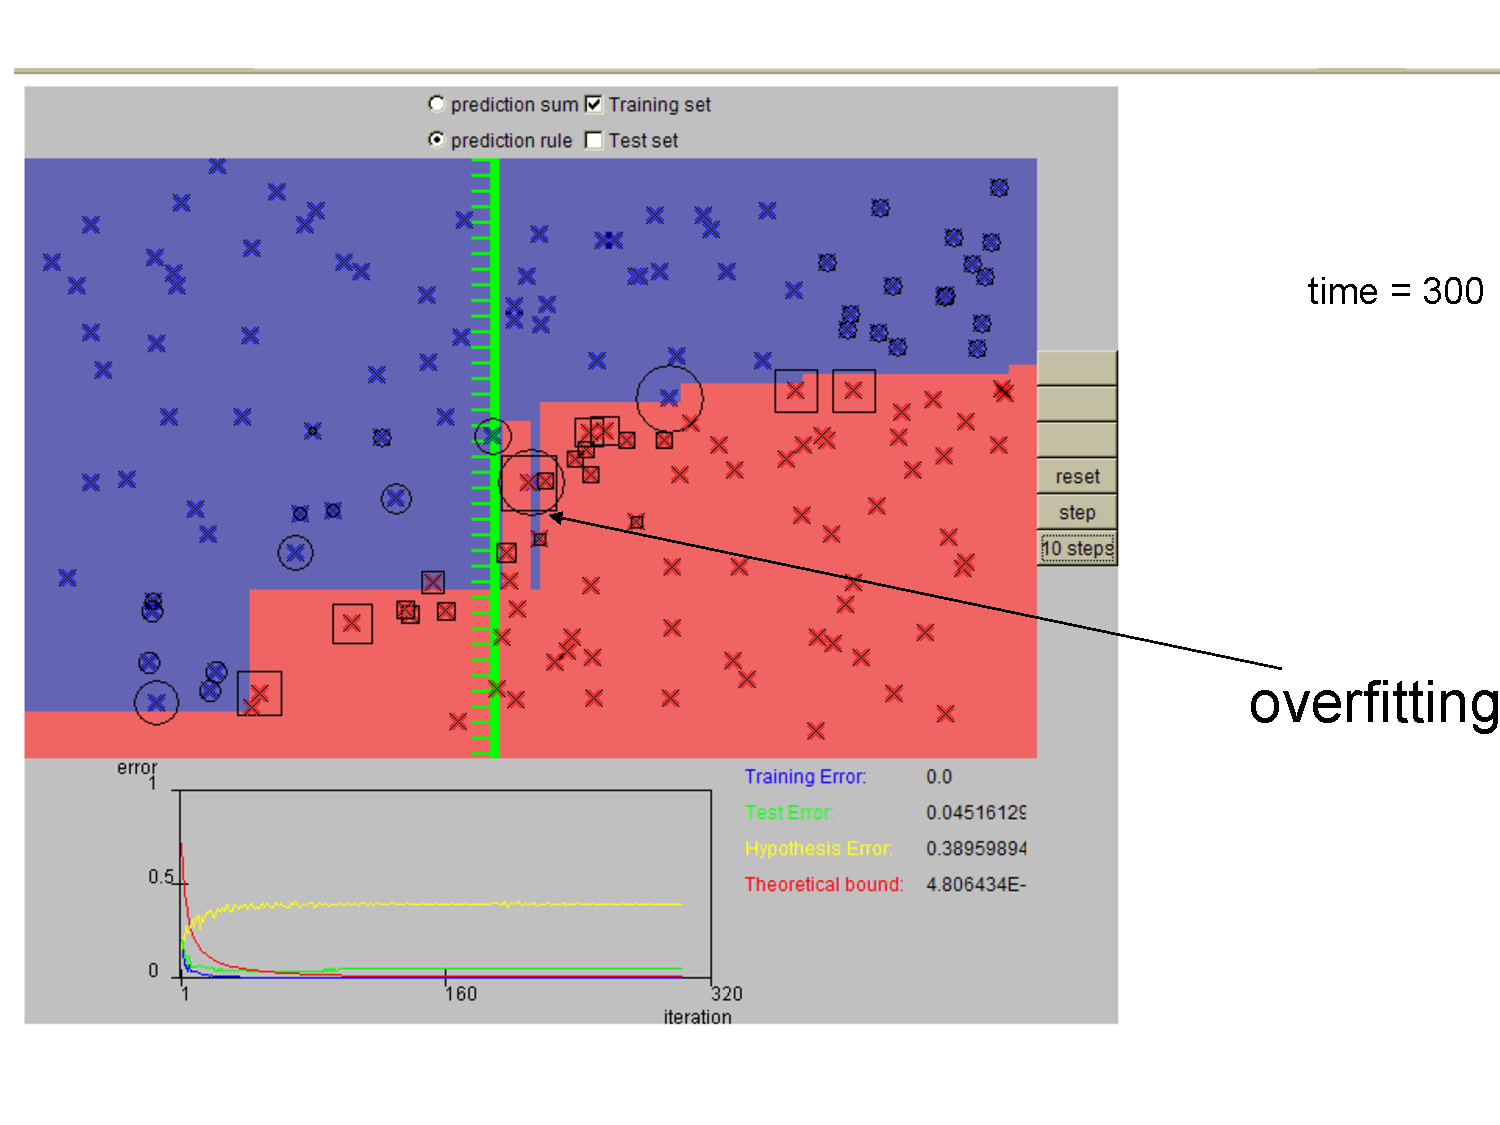
\includegraphics[width=2.5in]{figures/bagging_example.pdf}  \hfill \\
After making 300 classifiers, we can get a step-like decision boundary.  
Stopping at 100 would have been better; it is not over-fit (not shown).  \hfill \\

The blue, green, yellow, and red lines:   % I e-mailed the forum to figure this out. 
\begin{itemize}
	\item blue = training error = same as usual.  Randomly choose a subset to hold-out for testing
	\item green = test error = same as usual.  Randomly choose a subset to hold-out for testing
	\item yellow = hypothesis error = the error of the new weak learner generated on that step 
			(i.e. a decision stump) \hfill \\
		"Last classifier we added was 38\% wrong. " 
		for time = 100 when Hypothesis error said 0.38
	\item red = theoretical bound = the bound on the training error, derived in the later slides
\end{itemize}
% TA: Training/test sets are selected as always: randomly choosing a subset to hold-out for testing. Hypothesis error tells you the error of the new weak learner generated on that step (i.e. a decision stump). Theoretical bound is the bound on the training error, derived in the later slides.

\subsubsection{Learning from weighted data}  
Consider a weighted data set: \hfill \\
\begin{itemize}
	\item $D(i)$ is the weight of the $i^{th}$ training example/point (not classifier!). 
		It gets bigger each time point $i$ is predicted incorrectly.  
		It doesn't get smaller, but you normalize (see below). 
		\hfill \\
		Point = $(\bm{x}^i, \bm{y}^i)$
	\item interpretations:
		\begin{itemize}
			\item the $i^{th}$ training example counts as if it occurred $D(i)$ times
			\item these extra counts mean that if we were to "resample" data, 
				we would get more samples of "heavier" data points. 
		\end{itemize}
	\item Now we always do weighted calculations:
		\begin{itemize}
			\item e.g. MLE for Naive Bayes
			\item redefine Count(Y=y) to be a weighted count: \hfill \\
				$\displaystyle Count(Y=y) = \sum_{j=1}^n D(j) \delta (Y^j = y)$
			\item ?? Is this counting the number of points we have right?? No.. what is it counting? 
			\item if point $j$ has been wrong many times before, 
					it becomes more important, as reflected by $D(j)$ being large. 
			\item setting $D(j) = 1$ (or any constant value!) for all $j$ recreates the unweighted case. 
		\end{itemize}
\end{itemize}


Note, we can use decision stumps for boosting.  Can also use logistic regression, but it isn't as easy to show as our clas stump example.  \hfill \\
\hfill \\

That's just about weighing the samples.  How do we weight the classifiers? 
We want to weight across \underline{all} data points. 
Use $\alpha$ to allow classifiers to have different votes. 

\subsubsection{Algorithm: Binary case}
\underline{Given}: points $(x^1, y^1), \dots, x^m, y^m$.  \hfill \\
For this case, $x^i \in \mathbb{R}$, and binary labels: $y^i \in \{-1, +1\}$ \hfill \\
\underline{Initialize}: $D_1(i) = 1/m$ for $i=1, \dot, m$.  \hfill \\
For $t = 1, \dots, T:$
\begin{itemize}
	\item Train base classifier $h_t(x)$ using $D_t$
	\item Chose the weight of importance for this classifier, $\alpha_t$. \hfill \\
		Note that this comes after training the classifier.  \hfill \\
		There are many possibilities for choosing $\alpha$, which are discussed later.  \hfill \\
	\item Update, for $i= 1 \dots m$:  \hfill \\
		$D_{t+1}(i) \propto D_t(i) exp(-\alpha_t y^i h_t(x^i))$ \hfill \\
				with normalization constant $\displaystyle \sum_{i=1}^M D_t(i) \exp(-\alpha_t y^i h_t(x^i))$ 
		\begin{itemize}
			\item The $D$ is getting reweighted for the next round.  \hfill \\
			What's happening inside: \hfill \\
			If $y^i h_t(x^i) > 0$, $h_i$ was correct.  \hfill \\
			But if $y^i h_t(x^i) < 0$, $h_i$ was wrong.  \hfill \\
			You multiply by $\alpha_t$, which can flip the sign inside the $\exp()$. \hfill \\
			If $h_i$ is correct and $\alpha > 0$, then $D_{t+1}(i) < D_t(i)$.  \hfill \\
			But if $h_i$ is wrong and $\alpha > 0$, then $D_{t+1}(i) > D_t(i)$.  \hfill \\
		\end{itemize}
	\item Output a final classifier: $\displaystyle h = sign \left( \sum_{i=1}^T \alpha_t h_t(x) \right)$ \hfill \\
		This is a linear sum of "base" (weak) classifier outputs. \hfill \\
		Note that $D$ is no longer in the picture. 		
\end{itemize}
If you had two classifiers, your result would be $\alpha_1 h_1 + \alpha_2 h_2$

\textbf{How to chose $\alpha$}: \hfill \\
First calculate $\displaystyle  \epsilon_t = \sum_{i=1}^m D_t(i) \delta(h_t(x^i \neq y^i)))$ \hfill \\
This is the error of $h_t$, weighted by $D_t$ \hfill \\
Then use $\displaystyle  \alpha_t = \frac{1}{2} \ln \left( \frac{1 - \epsilon_t}{\epsilon_t} \right)$  (derived below) \hfill \\
This transforms alpha according to:  \hfill \\
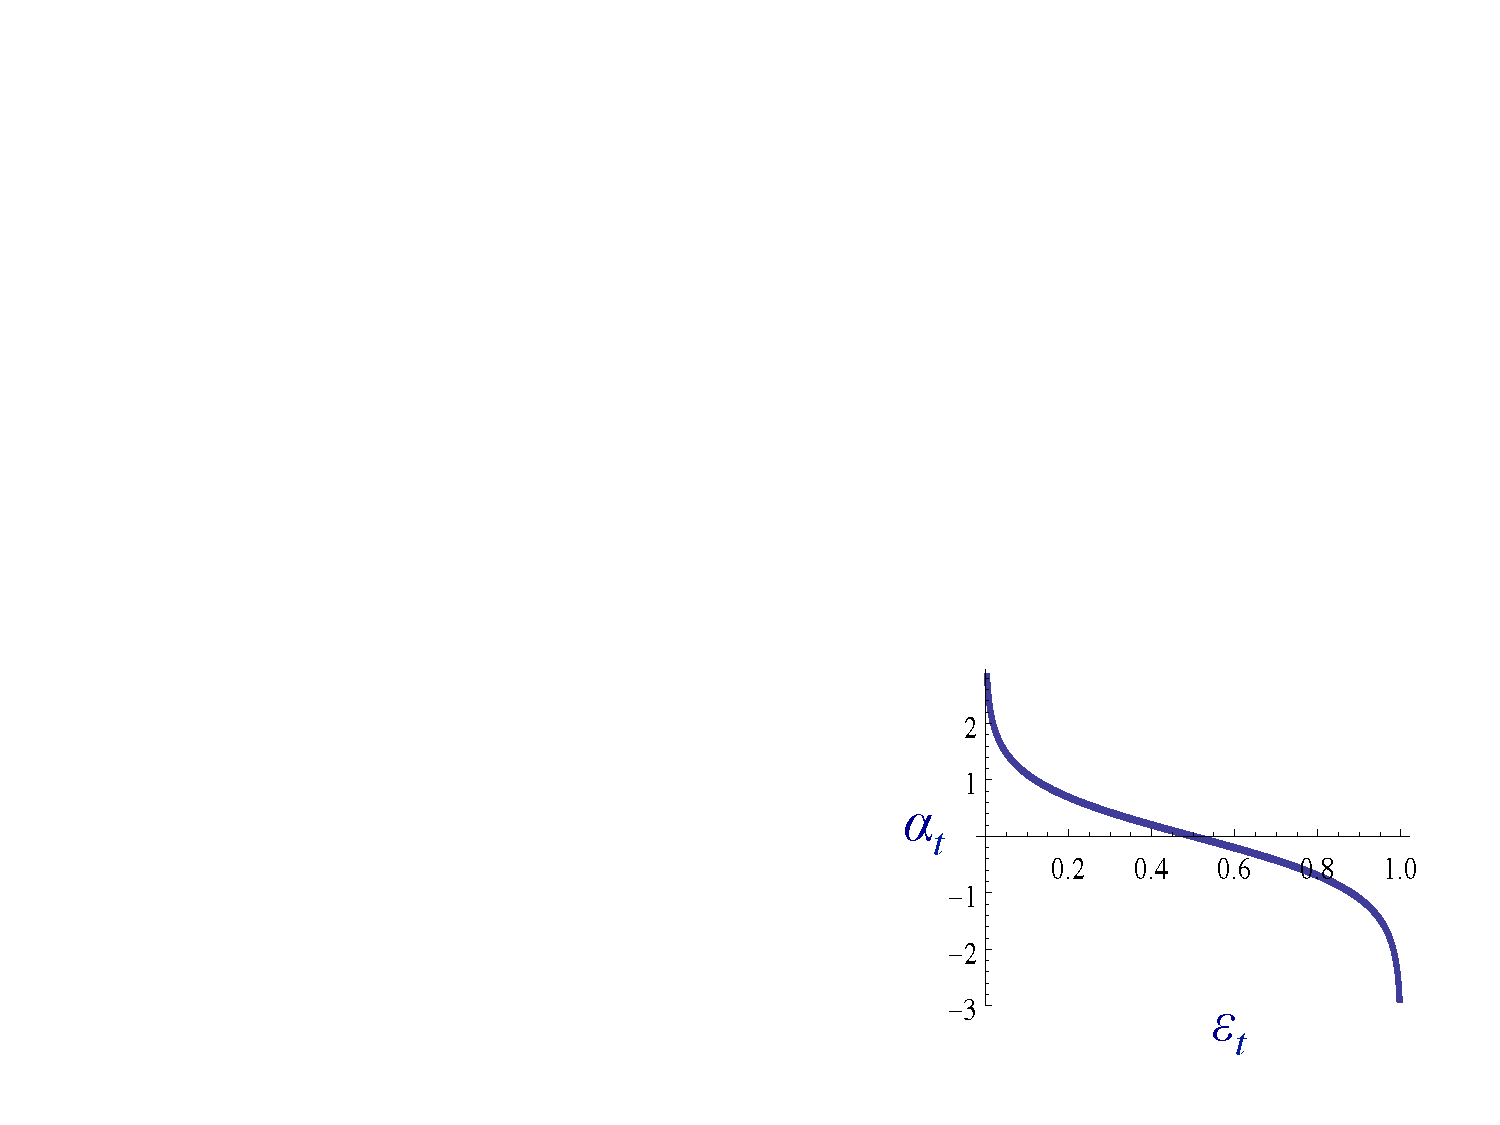
\includegraphics[width=1.2in]{figures/alpha_from_epsilon.pdf}
\begin{itemize}
	\item no errors:  $\epsilon_t = 0 \rightarrow \alpha_t = \infty$
	\item all errors:  $\epsilon_t = 1 \rightarrow \alpha_t = -\infty$
	\item random:  $\epsilon_t = 0.5 \rightarrow \alpha_t = 0$
\end{itemize}
Truncate at 2 or 3.  Don't want to allow weight = infinity. \hfill \\  % week 9 audio
Think of this like NB with weighting. \hfill \\  % week 8 audio.
\underline{Why would we want/have negative weights on classifiers?} \hfill \\
A classifier that does worse than chance is backwards. 
If it is worse than chance, flip the sign then use it. 
A classifier that is wrong 90\% of the time is a good classifier.   
A truly random classifier does not provide information.  Thow those away.

\hfill \\
If you get something right a bunch of times, the weight should converge to zero.  % week 8 audio
\hfill \\

We want to run this loop until it converges.  
But if we run it too long, it will overfit. 

\subsubsection{How to chose $\alpha_t$ for hypothesis $h_t$?}
It would be cool to find the $\alpha_t$ that works best for that classifier, take derivative with respect to $\alpha_t$, and find an $\alpha$ that minimizes error. \hfill \\
We can't optimize the training set error, but we can minimize a bound on it. \hfill \\
$\displaystyle  \sum_{i=1}^m \delta(H(x^i) \neq y^i) \leq \sum_{i=1}^m D_t(i) \exp(-y^i f(x^i))$ \hfill \\
where $\displaystyle f(x) = \sum_t \alpha_t h_t(x)$; $H(x) = sign(f(x))$ \hfill \\
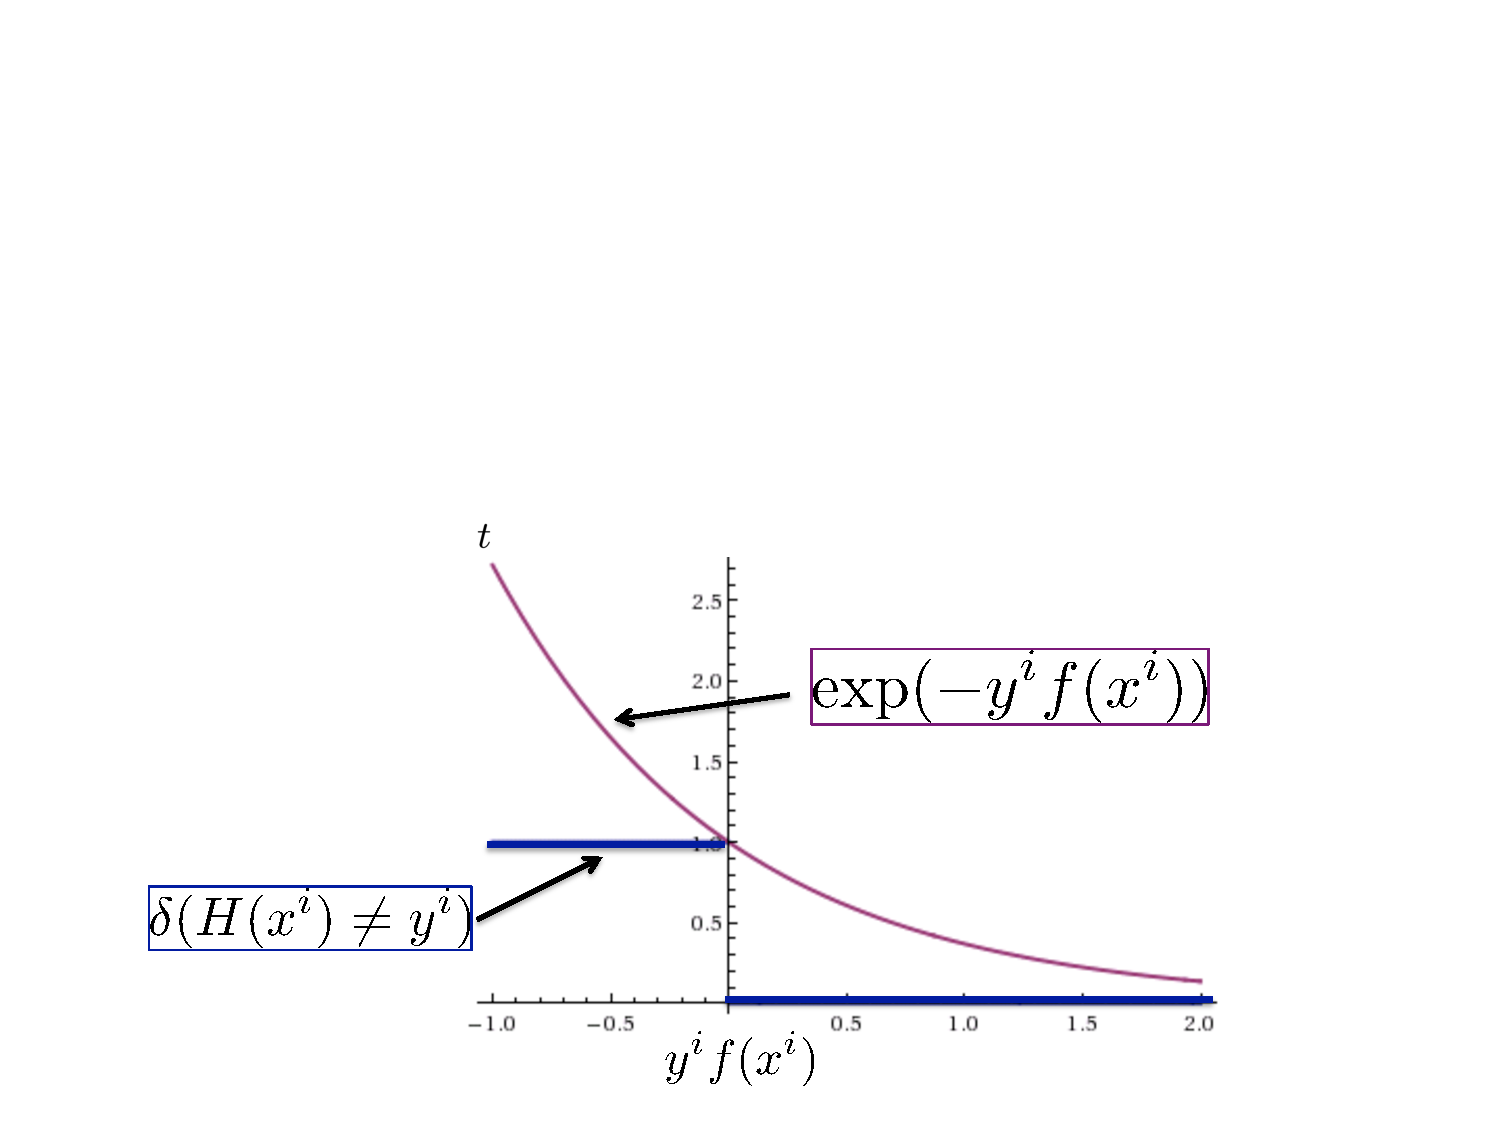
\includegraphics[width=2.5in]{figures/chosing_alpha_step_func.pdf}
 
We know the training set error (\# of instances wrong) it is bounded by the sum on the right.
Why?  The left side of the equality is the left piece of the step function.
The exponential function of label*prediction has the expo curve.
Note that \textbf{the exponential curve is always above the step function}.
So we can use expo as the upper bound. 
This is kind of like logistic regression: same form.

% --------
\subsubsection{You can choose $\alpha_t$ to minimize the error bound.}
Note that each classifier is independent of alpha.  
Each classifier is already a classifier by itself. 
We want to train the weighted combinations of classifiers.  
Note we are not directly using the error.  
We are using a function that maps the error to a \# we can use. 
That's the role of the alpha vs epsilon curve.  
We liked its properties. 
There are two parameters in the $\exp()$:  $h$ and $\alpha.$
You can optimize for h and alpha together.
We have a way to make the classifier sand learn the weights at the same time.
We might still learn the classifiers first. 
For those of you who care about joint optimization, you can flip between optimizing the two. 

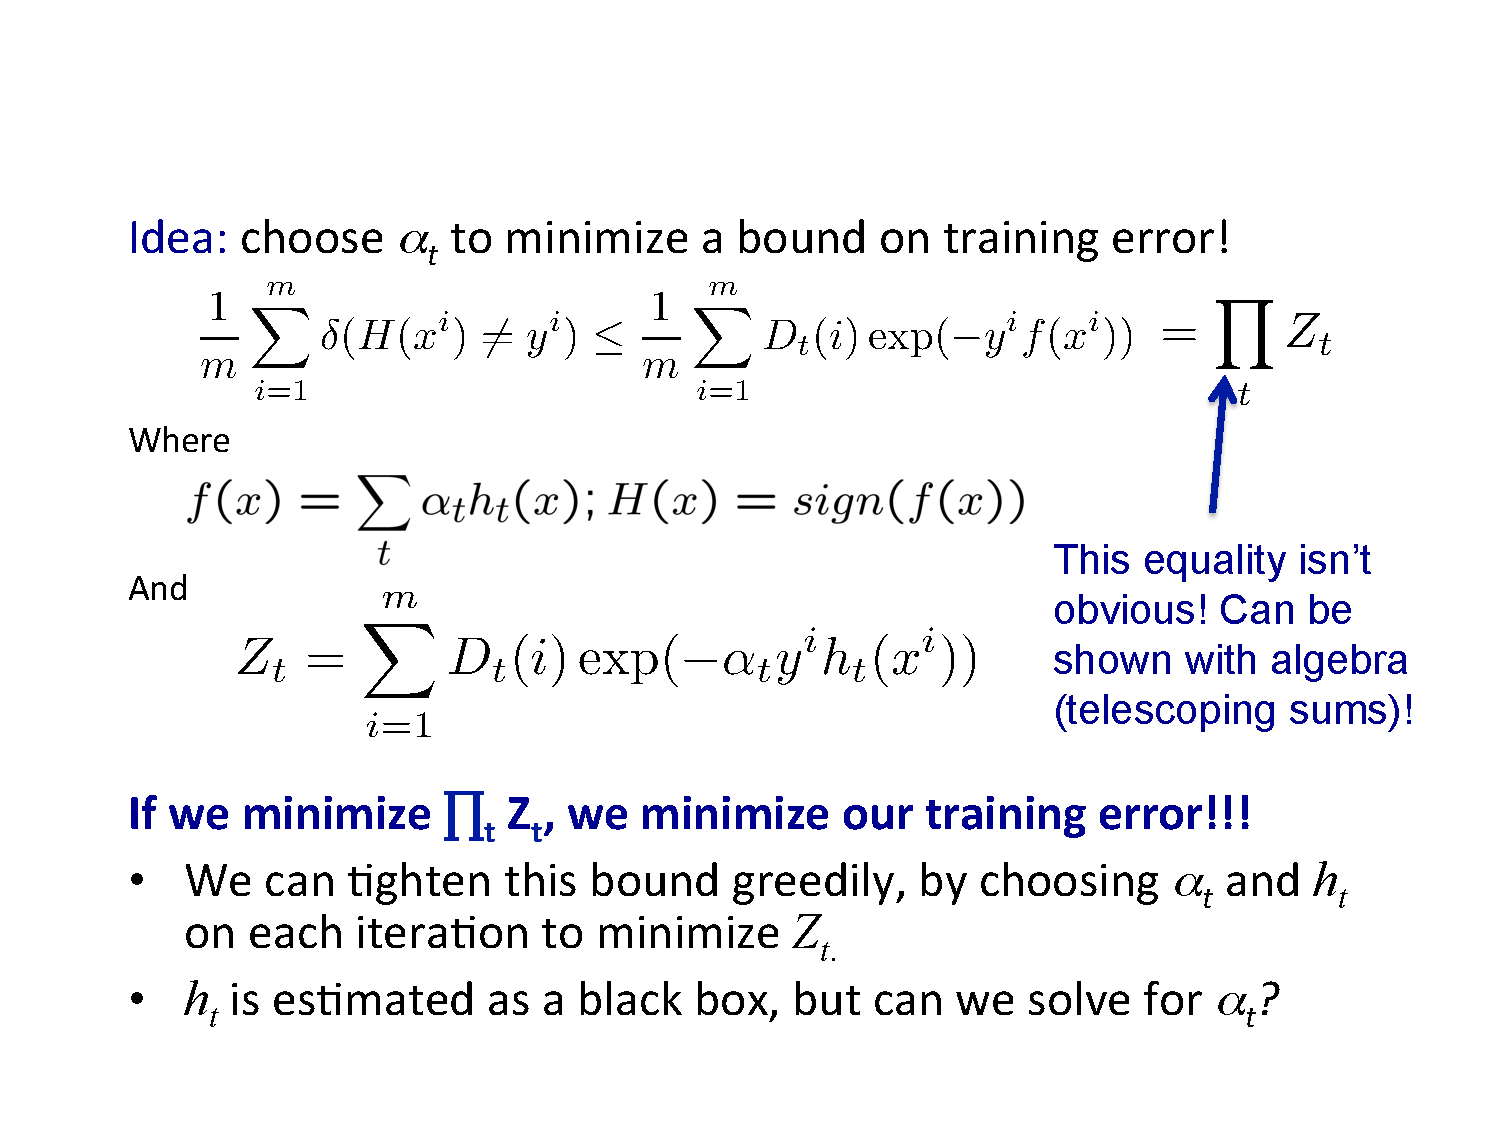
\includegraphics[width=2.7in]{figures/chosing_alpha--telescoping_sums.pdf}

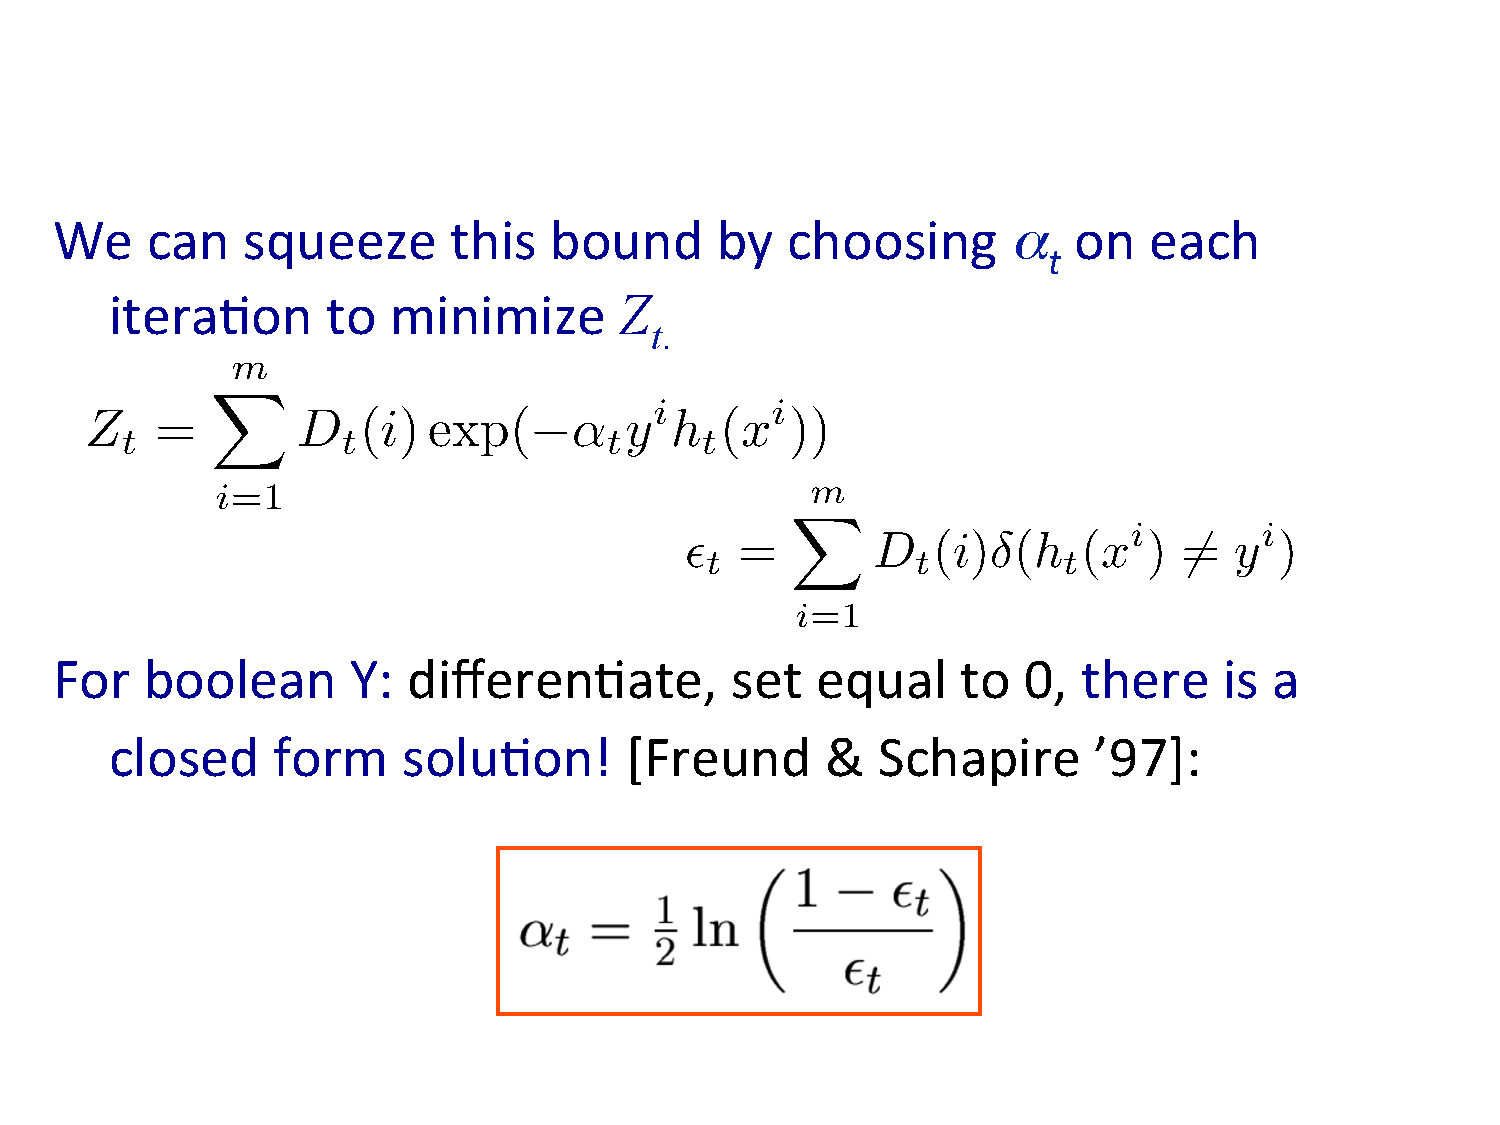
\includegraphics[width=2.7in]{figures/chosing_alpha--telescoping_sums2.pdf}

Note that our $D$ values are not going up by more than 1 each time, like the intro to the concept showed.
There is an exponential term that generally shrinks the sum of the $D$ values to 1 (at least in the class example).  \hfill \\
\hfill \\

After the third iteration for our class example:
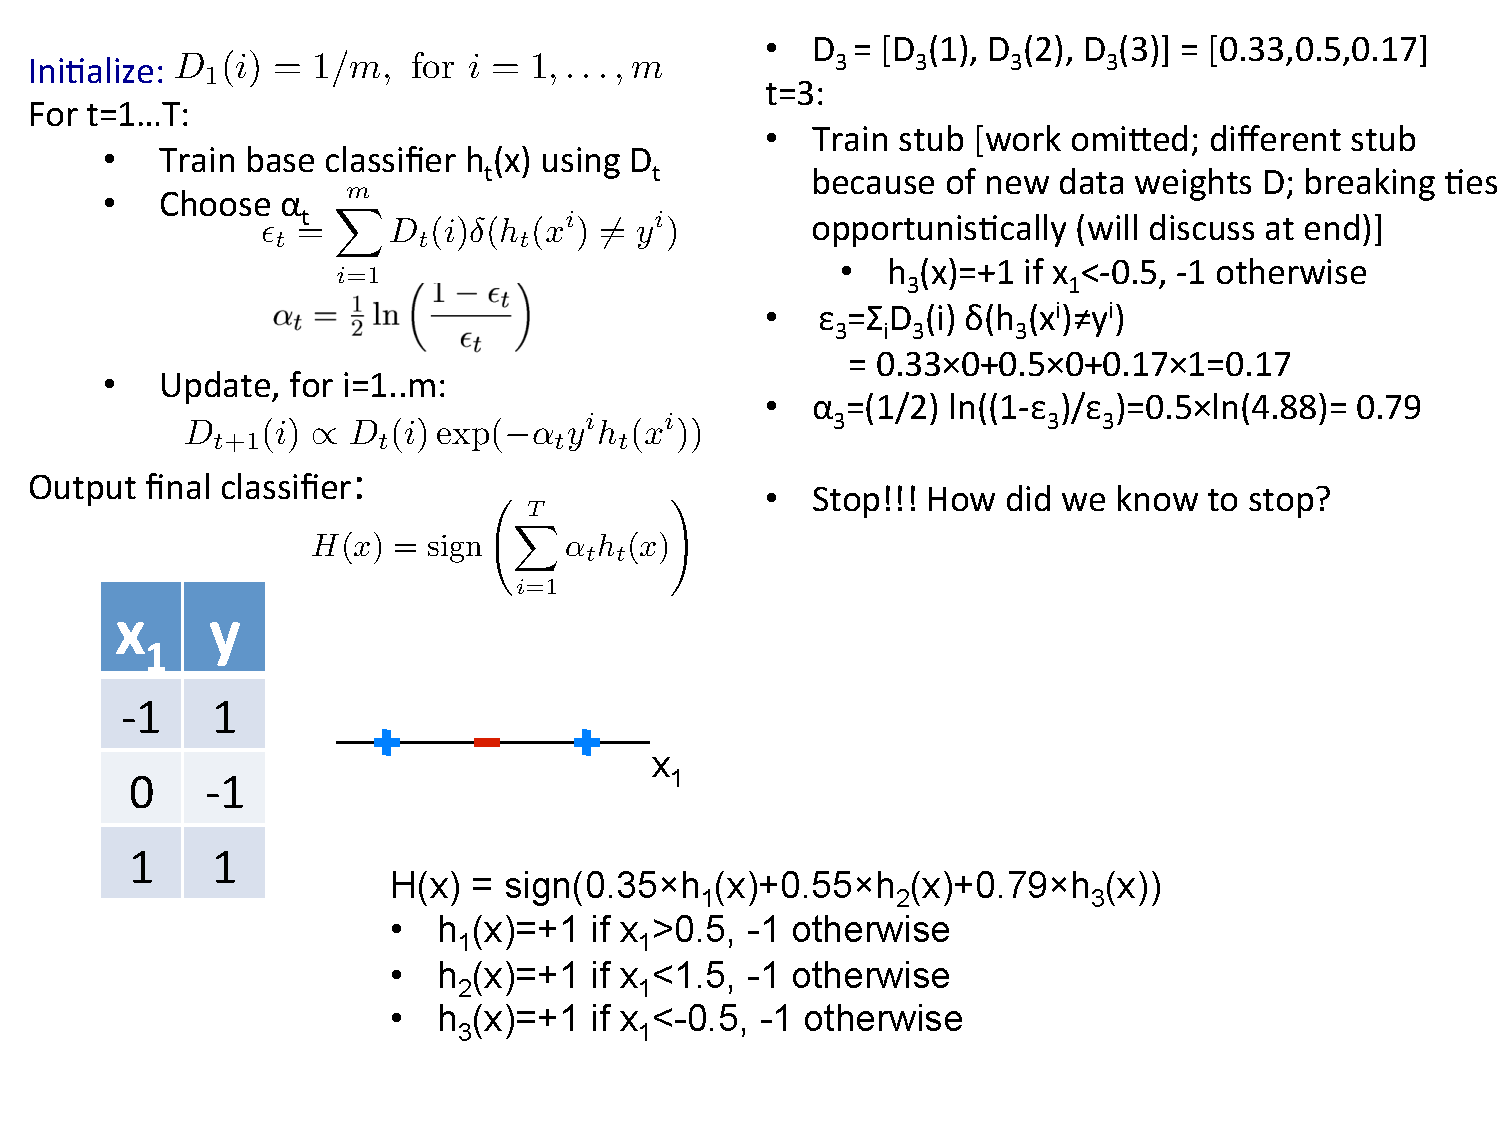
\includegraphics[width=3.4in]{figures/boosting_example_3rd_iteration.pdf} \hfill \\
The $\epsilon$ values are dependent on the previous iteration's $D$ values, 
	but the current iterations $h$ classifier. \hfill \\
Once you find your new $\epsilon$ from your old $D$s and new $h$, 
	you can find $\alpha$ and thus your new $D$s for the next round.   \hfill \\
%?? Does your previous classifier know anything about your other classifiers ??    \hfill \\
%?? Should we think of the fact that it was trained using $D$s from previous classifiers as knowledge about other classifiers ??   \hfill \\
?? Is it typical to have your alpha weights grow ??  Can I explain what is driving this ?? 
\hfill \\
\hfill \\

\textbf{The D after normalization is a probability.}

\subsubsection{Assembling weak classifiers}
If each classifier is (at least slightly) better than random: $\epsilon_t < 0.5$: \hfill \\
Another bound on error:
$$ \frac{1}{m} \sum_{i=1}^m \delta (H(x^i) \neq y^i) \leq \prod_t Z_t \leq \exp \left( -2 \sum_{t=1}^T (\frac{1}{2} - \epsilon_t)^2 \right)$$
This implies training error will reach zero exponentially fast. \hfill \\
The error is bounded by an exponential of how far you are from random. \hfill \\

Note that it isn't too hard to achieve better than random training error, especially for binary classification.   \hfill \\
Boosting is powerful!  \hfill \\

Note that test error can continue to decrease after training error goes to zero.  

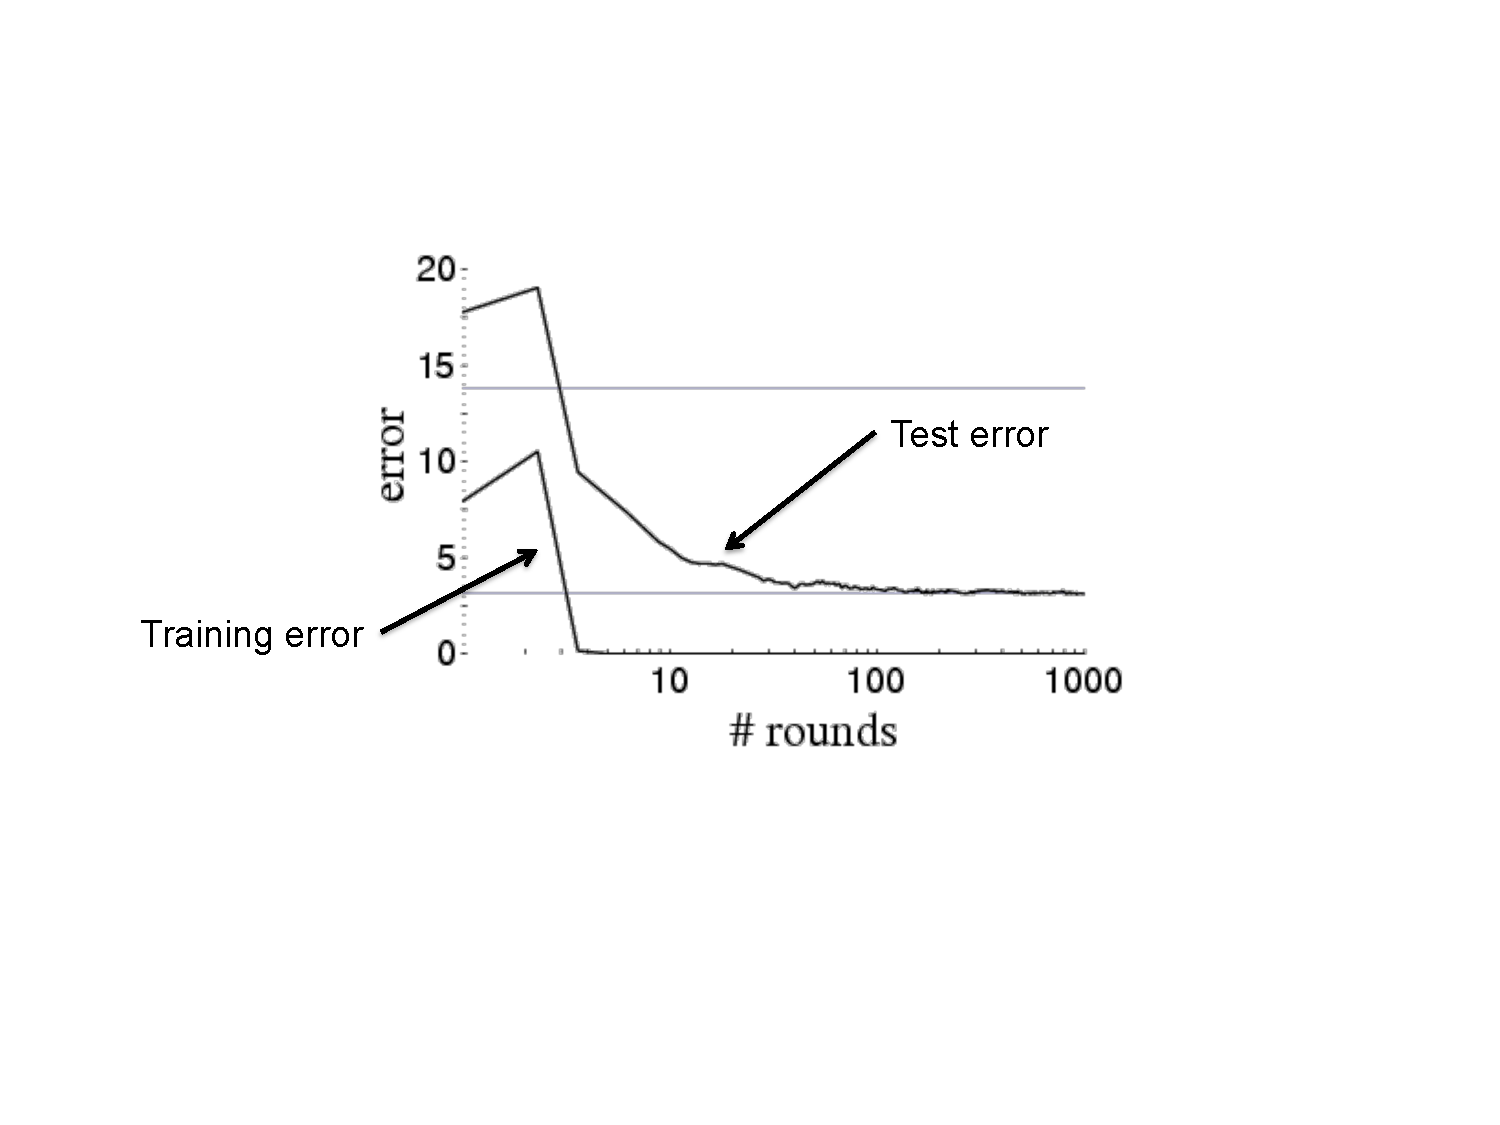
\includegraphics[width=2.2in]{figures/boosting_train_test_error.pdf}

Also in this figure, the lack of up-tick at the right shows that boosting does not overfit. 

\subsubsection{Using your classifier}
Say you have a trained/converged classifier.
That means you have $h$s and $\alpha$s : weak classifiers and their corresponding weights. 
Plug in new $x$ into $H(x)$ %, which puts into $H(x)$.

\textbf{How do we know when to stop? } \hfill \\
If the training error keeps getting better we keep going.
This could lead to over-fitting, but it turns out boosting is robust to overfitting.   \hfill \\
(We didn't actually conclude when to stop in class.) 

There was a theory (Freund \& Schapire, 1996) that suggested 
$$ error_{true}(H) \leq error_{train}(H) + \tilde{\mathcal{O}} \left( \sqrt{\frac{Td}{m}} \right) $$
Suggests you don't want to use complicated classifiers in your boosting.  d would get high, we could end up over-fitting. % week 9 audio

$T$: number of boosting rounds.  Higher $T$ $\rightarrow$ looser bound.  \hfill \\
$d$: VC dimension of weak learner.  Measures complexity of classifier.  \hfill \\
$m$: number of training examples.  More data $\rightarrow$ tighter bound.  \hfill \\
\hfill \\

It turns out boosting is robust to overfitting.  The test set error decreases even after the training error reaches zero.  So this theory doesn't hold. 

\subsubsection{Boosting and Logistic Regression}
Both smooth approximations of 0/1 step loss.

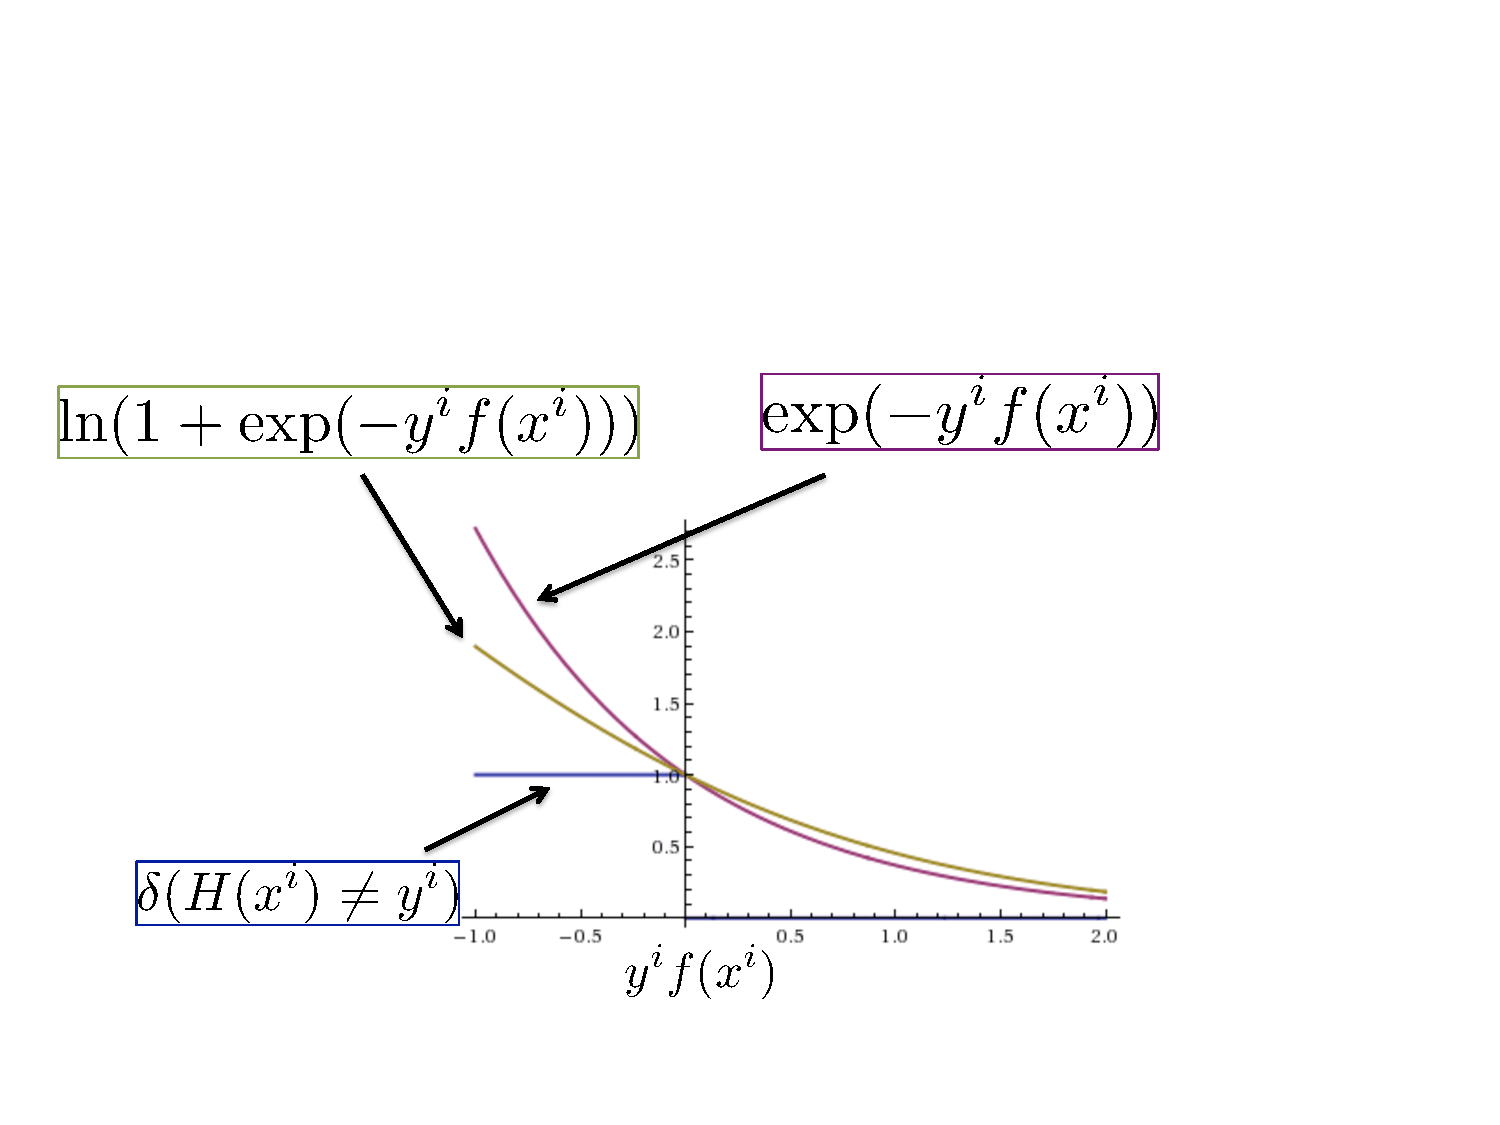
\includegraphics[width=2.2in]{figures/losses--boosting_and_logistic_regression.pdf}

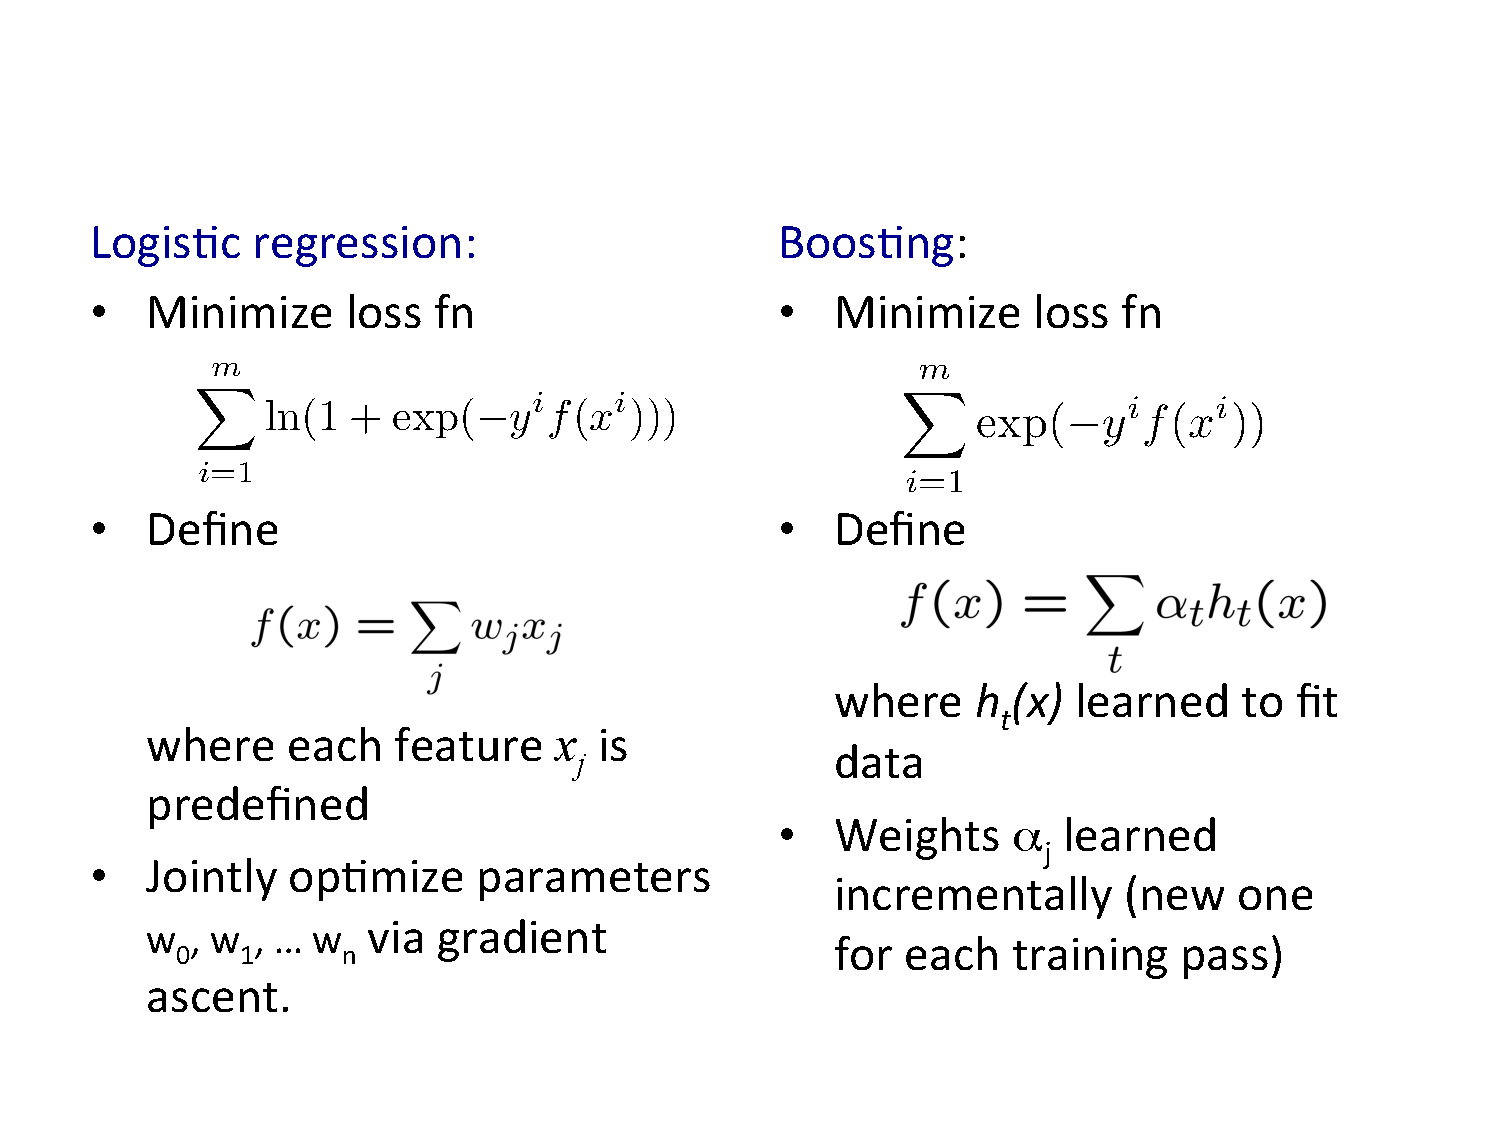
\includegraphics[width=2.7in]{figures/logistic_regression_and_boosting_summary.pdf}

As noted above:
Similar to logistic regression:
\begin{itemize}
	\item both linear models.  Boosting "learns" features.  
	\item similar loss functions
	\item single optimization (Logistic Regression) versus incrementally improving
\end{itemize} 

